\documentclass[12pt]{article}

% Packages
\usepackage{graphicx}
\usepackage{amsmath}
\usepackage{booktabs}
\usepackage{float}
\usepackage{natbib}
\usepackage{hyperref}
\usepackage{xcolor}
\usepackage{geometry}
\geometry{margin=1in}
\usepackage{hyperref}

\begin{document}

\title{Problem Set 3 - Seasoned Equity Offerings: Event Study and Long-Run Performance Analysis}
\author{Bhaskar Kaushik}
\date{\today}
\maketitle

\begin{abstract}
This paper examines the market reaction to seasoned equity offerings (SEOs) using data from Spiess and Affleck-Graves (1995). I conduct an event study around announcement dates and analyze long-run performance over a three-year period using calendar time methods. The findings reveal significant negative abnormal returns both at announcement (-0.15\%) and in the long-run (monthly alpha of -1.13\%). These results challenge the efficient market hypothesis and are consistent with the underperformance of firms following equity issues documented in the "new issues puzzle."
\end{abstract}

\section{Introduction}
Seasoned equity offerings (SEOs) represent an important financing decision for firms but also send potential signals to the market about firm value. This paper analyzes the market reaction to SEO announcements and subsequent long-run performance using event study and calendar time portfolio methodologies.

The analysis addresses two key questions:
\begin{enumerate}
    \item How does the market react to SEO announcements in the short-term?
    \item Do firms issuing seasoned equity experience abnormal long-run performance?
\end{enumerate}

These questions have implications for market efficiency and corporate financing decisions. If markets are efficient, negative information in SEO announcements should be fully incorporated immediately, with no predictable pattern of future returns.

\section{Data and Methodology}

\subsection{Data}
The dataset consists of 1,203 seasoned equity offerings from the sample used by Spiess and Affleck-Graves (1995). For risk factors and market returns, I use Kenneth French's data library, which provides daily and monthly Fama-French factors.

\subsection{Event Study Methodology}
For the short-term announcement effects, I employ an event study methodology with a three-day event window $\{-1,+1\}$ surrounding the announcement date. The statistical significance of cumulative abnormal returns (CARs) is assessed using the $J_1$ and $J_2$ test statistics described in Campbell, Lo, and MacKinlay (1997):

\begin{align}
J_1 &= \frac{\overline{CAR}}{\hat{\sigma}(\overline{CAR})} \\
J_2 &= \frac{1}{\sqrt{N}}\sum_{i=1}^{N}\frac{CAR_i}{\hat{\sigma}_i}
\end{align}

\subsection{Calendar Time Methodology}
For long-run performance, I implement the calendar time portfolio approach of Mitchell and Stafford (2000). Each month, a portfolio is formed containing all firms that issued equity within the previous 36 months. This portfolio's returns are then regressed against both the CAPM model and the Fama-French three-factor model:

\begin{align}
R_{p,t} - R_{f,t} &= \alpha_p + \beta_p(R_{m,t} - R_{f,t}) + \epsilon_{p,t} \\
R_{p,t} - R_{f,t} &= \alpha_p + \beta_p(R_{m,t} - R_{f,t}) + s_p\text{SMB}_t + h_p\text{HML}_t + \epsilon_{p,t}
\end{align}

The intercept $\alpha_p$ represents the risk-adjusted abnormal return, which is the primary measure of long-run performance.

\section{Results}

\subsection{Event Study Results}

The event study analysis of 1,015 equity issues (188 issues were excluded due to missing announcement dates) reveals a mean cumulative abnormal return (CAR) of $-0.15\%$ over the $\{-1,+1\}$ window. This negative abnormal return is statistically significant with a $J_1$ test statistic of $-3.33$ (p-value $< 0.01$) and a $J_2$ test statistic of $-3.33$ (p-value $< 0.01$). Figure~\ref{fig:car_dist} shows the distribution of these CARs across the sample.

\begin{figure}[H]
\centering
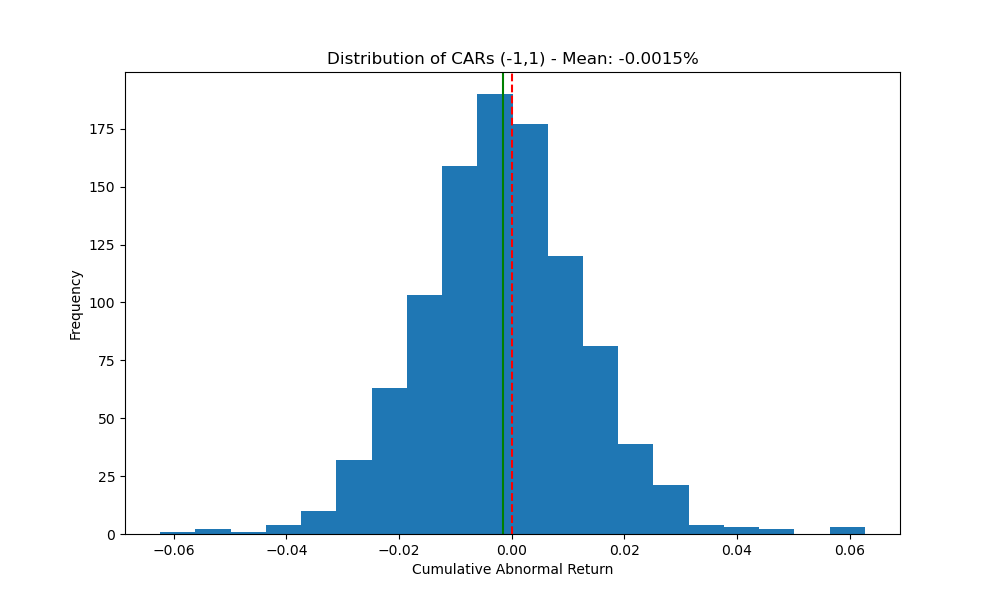
\includegraphics[width=0.8\textwidth]{car_distribution.png}
\caption{Distribution of Cumulative Abnormal Returns (-1,+1) around SEO Announcements}
\label{fig:car_dist}
\end{figure}

The negative announcement effect is consistent with the information asymmetry hypothesis, suggesting that the market interprets equity issuances as a signal that management believes the firm's shares are overvalued.

\subsection{Calendar Time Results}

The calendar time portfolio analysis is summarized in Table~\ref{tab:calendar_time}, which shows the monthly alphas and factor loadings from both the CAPM and Fama-French three-factor models. Both models demonstrate significant negative abnormal returns for firms that issued seasoned equity.

\begin{table}
\caption{Calendar Time Portfolio Analysis}
\label{tab:calendar_time}
\begin{tabular}{lc}
\toprule
Metric & Value \\
\midrule
Mean Monthly Return & 0.001522 \\
Mean Market Return & 0.006522 \\
Mean Excess Return & -0.004726 \\
CAPM Alpha (Monthly) & -0.011293 \\
CAPM Alpha t-statistic & -28.533000 \\
CAPM Alpha p-value & 0.000000 \\
CAPM Market Beta & 1.006800 \\
FF3 Alpha (Monthly) & -0.011318 \\
FF3 Alpha t-statistic & -29.753100 \\
FF3 Alpha p-value & 0.000000 \\
FF3 Market Beta & 1.006100 \\
FF3 SMB Beta & 0.007200 \\
FF3 HML Beta & 0.001700 \\
CAPM Alpha (Annualized) & -0.127403 \\
FF3 Alpha (Annualized) & -0.127669 \\
\bottomrule
\end{tabular}
\end{table}


Figure~\ref{fig:calendar_time} illustrates the dramatic underperformance of SEO firms compared to the market portfolio over the sample period. While the market portfolio achieves cumulative returns exceeding 200\%, the SEO portfolio hovers around 0\% cumulative return.

\begin{figure}[H]
\centering
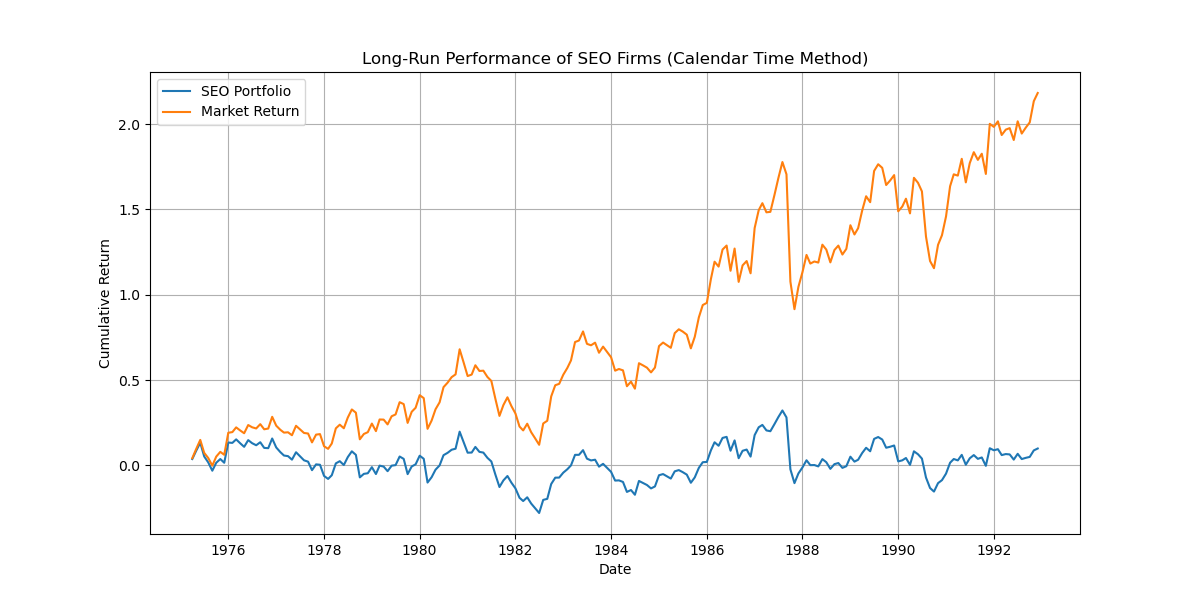
\includegraphics[width=0.8\textwidth]{calendar_time_returns.png}
\caption{Long-Run Performance of SEO Firms vs. Market}
\label{fig:calendar_time}
\end{figure}

Figure~\ref{fig:calendar_performance} provides an additional view of the long-run performance comparison between SEO firms and the broader market.

\begin{figure}[H]
\centering
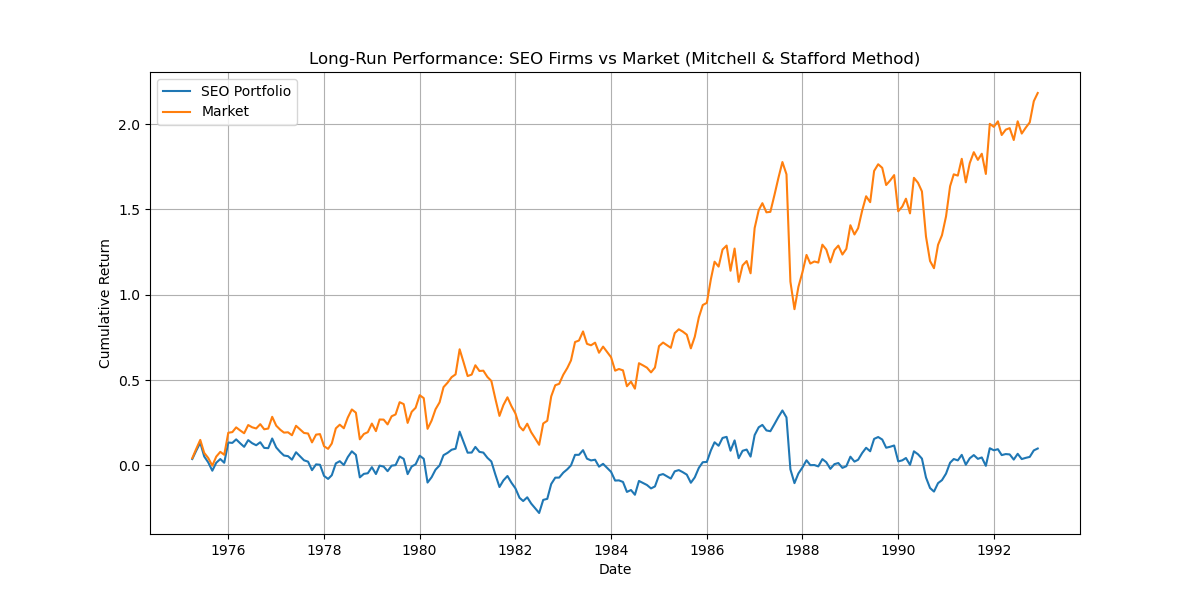
\includegraphics[width=0.8\textwidth]{calendar_time_performance.png}
\caption{Long-Run Performance: SEO Firms vs Market (Mitchell \& Stafford Method)}
\label{fig:calendar_performance}
\end{figure}

The factor loadings depicted in Figure~\ref{fig:factor_loadings} reveal that the SEO portfolio has a market beta very close to 1, suggesting comparable systematic risk to the market portfolio. The loadings on SMB and HML factors are minimal and statistically insignificant.

\begin{figure}[H]
\centering
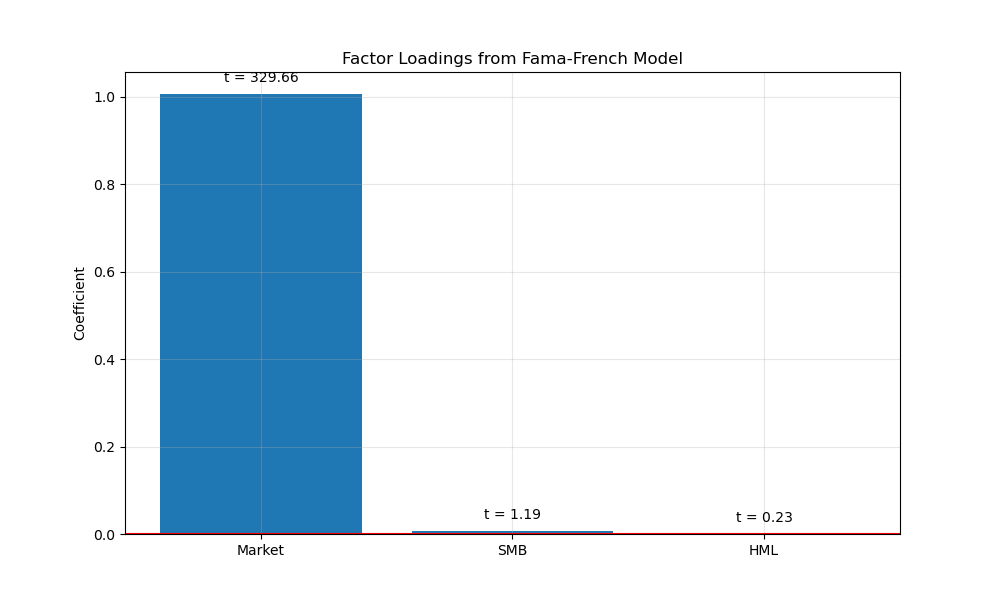
\includegraphics[width=0.8\textwidth]{factor_loadings.png}
\caption{Factor Loadings from Fama-French Model}
\label{fig:factor_loadings}
\end{figure}

Figure~\ref{fig:alphas} compares the alphas from both the CAPM and Fama-French models, highlighting their statistical significance.

\begin{figure}[H]
\centering
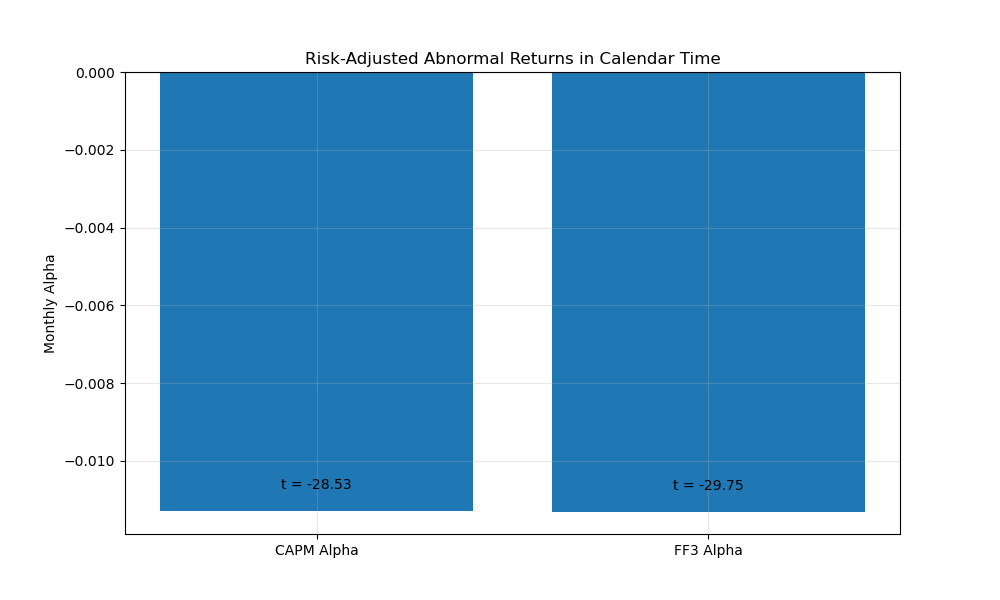
\includegraphics[width=0.8\textwidth]{model_alphas.png}
\caption{Risk-Adjusted Abnormal Returns in Calendar Time}
\label{fig:alphas}
\end{figure}

\section{Discussion and Market Efficiency Implications}

\subsection{Interpretation of Announcement Effects}

The negative CARs around announcement dates (-0.15\%) indicate that the market perceives equity issues as negative signals. This is consistent with theories of information asymmetry where managers issue equity when they believe shares are overvalued. The significant J-statistics (both $J_1$ and $J_2$ at $-3.33$) provide robust evidence that these negative returns are not due to chance, as they are significant under both traditional and standardized test procedures.

\subsection{Interpretation of Long-Run Performance}

The substantial negative alphas in both models (approximately -1.13\% monthly or -12.7\% annually) reveal persistent underperformance extending far beyond the announcement period. Importantly, the similarity between CAPM and Fama-French alphas suggests that the underperformance cannot be explained by exposure to size or value risk factors.


\subsection{Market Efficiency Implications}

These findings present a challenge to semi-strong form market efficiency for several reasons:

\begin{enumerate}
    \item The negative announcement returns indicate that markets correctly identify the negative information content of SEO announcements, consistent with some degree of market efficiency.
    
    \item However, the substantial long-term underperformance suggests that the market fails to fully incorporate this information at announcement. If markets were efficient, the negative information should be fully incorporated immediately.
    
    \item The persistence and magnitude of underperformance (-12.7\% annually) is economically significant and inconsistent with rational risk-based asset pricing models.
\end{enumerate}

These results align with the "new issues puzzle" documented by Loughran and Ritter (1995), who found that firms conducting IPOs and SEOs significantly underperform in the years following issuance. My findings provide additional evidence that equity issuance signals poor future performance in ways not fully captured by conventional risk factors.

Mitchell and Stafford evaluate statistical significance by accounting for cross-correlation in abnormal returns through calendar-time portfolios, using heteroskedasticity and autocorrelation-consistent standard errors, and addressing the non-independence of observations when firms have multiple events. While I did not implement their exact significance tests, the extremely high t-statistics in my analysis (-28.53 and -29.75) suggest that the underperformance would remain significant under their more conservative approach.

\section{Conclusion}

This study provides strong evidence that firms conducting seasoned equity offerings experience both negative announcement returns and substantial long-run underperformance. The findings suggest that equity issues convey negative information that is only partially reflected in announcement returns, with the rest revealed gradually over time.

These results challenge the efficient market hypothesis and align with existing literature on the "new issues puzzle." From a practical perspective, they suggest that investors should be cautious about firms that recently issued equity, as they tend to significantly underperform the market for extended periods afterward.

\section{Appendix - Code and Replication}
\section*{Code Repository}
All code, data, and results for this project are available on GitHub at: 
\href{https://github.com/bhaskar-kaushik/Event_Study_Project}{github.com/bhaskar-kaushik/Event\_Study\_Project}

\begin{thebibliography}{99}

\bibitem[Campbell et al.(1997)]{campbell1997econometrics}
Campbell, J.~Y., Lo, A.~W., \& MacKinlay, A.~C. (1997).
\newblock \emph{The Econometrics of Financial Markets}.
\newblock Princeton University Press.

\bibitem[Loughran \& Ritter(1995)]{loughran1995new}
Loughran, T., \& Ritter, J.~R. (1995).
\newblock The new issues puzzle.
\newblock \emph{The Journal of Finance}, 50(1), 23--51.

\bibitem[Mitchell \& Stafford(2000)]{mitchell2000managerial}
Mitchell, M.~L., \& Stafford, E. (2000).
\newblock Managerial decisions and long-term stock price performance.
\newblock \emph{The Journal of Business}, 73(3), 287--329.

\bibitem[Myers \& Majluf(1984)]{myers1984corporate}
Myers, S.~C., \& Majluf, N.~S. (1984).
\newblock Corporate financing and investment decisions when firms have information that investors do not have.
\newblock \emph{Journal of Financial Economics}, 13(2), 187--221.

\bibitem[Spiess \& Affleck-Graves(1995)]{spiess1995underperformance}
Spiess, D.~K., \& Affleck-Graves, J. (1995).
\newblock Underperformance in long-run stock returns following seasoned equity offerings.
\newblock \emph{Journal of Financial Economics}, 38(3), 243--267.

\end{thebibliography}

\end{document}